\chapter{The Atoms} \label{ChapterAboutTheAtoms}
\section{Overview of relevant atomic transitions}

The system is designed to stimulate Raman transitions between the hyperfine $^2$S$_{1/2}$ ($5s$) ground states corresponding to $F=4$ and $F=5$. The intermediate state is the $^2$P$_{3/2}$ ($5p$) state. 

\begin{figure}
\centerline{
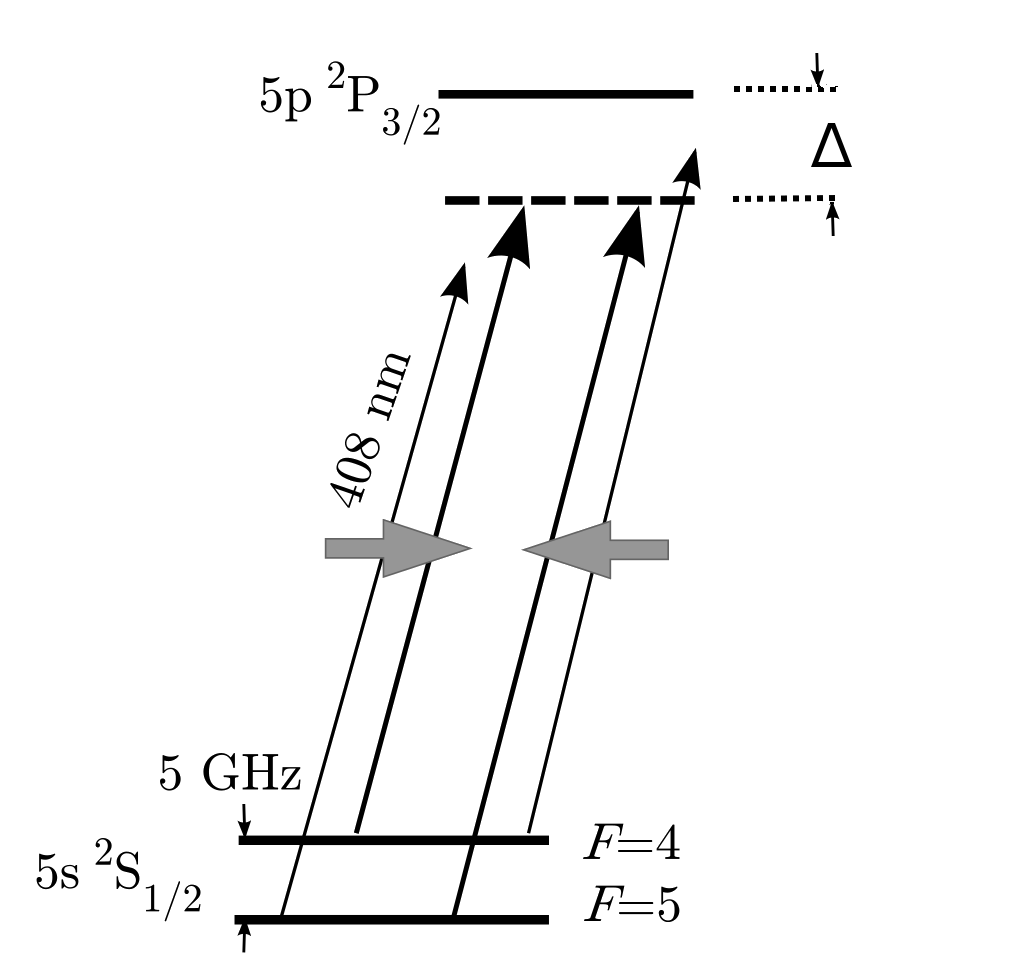
\includegraphics[totalheight=0.3\textheight]{E_level_from_proposal}
}
\caption[Energy Level Diagram for $^{87}$Sr+]{Energy Level Diagram for $^{87}$Sr+. The hyperfine ground states are separated by a small energy. Diagram is not to scale: a scaled diagram would show the splitting between the $F=4$ and $F=5$ states to be about 147,000 times smaller than the splitting between the $^2$S$_{1/2}$ states and the $^2$P$_{3/2}$ states.}
\end{figure}

Our objective in this chapter is to calculate the necessary intensity and beam waist that will allow our lasers to impart the $\pi$ and $\pi/2$ pulses to the atoms as they make their way through the chamber. In order to do this, we first review the various relevant states of this atom and the quantum numbers used to describe them. Then we move onto a discussion of some of the basic aspects of hyperfine structure. We will then model the atom as a three state system and obtain an expression relating the magnitude and frequency of the electric field to the Rabi frequencies of our two transitions. Finally, we calculate the total transition rate for the 3 state system and we tabulate the beam parameters that will produce the requisite electric field strengths for the correct amounts of time to produce the transition.

The discussion that follows is for calculating the transition amplitudes using values of physical parameters found in the literature.

In Ref.\ \cite{cjeDiss}, this calculation is performed, but some of the details are left mysterious. In particular, no source is cited for any of the physical parameters of the $^{87}$Sr+ atom (e.g. the dipole moment values, the transition width, the saturation parameter). We hope to reproduce this calculation with more details.  

\section{States and Quantum Numbers}

The Hamiltonian of the Strontium ions is analagous to the Hamiltonian of a single-electron atom. 
In a single electron atom, the solution to the Schr\"odinger equation describing the electron is solved by separation of variables.
 Each solution is a product of a spherically symmetric function that depends only on the distance $r$ from the nucleus and the spherical harmonics.
This is because the orbital angular momentum operator $\mathbf{L}$ commutes with such a Hamiltonian. In fact, the orbital angular momentum operator commutes with any Hamiltonian with a spherically symmetric potential.
Thus, we can use the familiar angular momentum quantum numbers for the eigenstates of any spherically symmetrical Hamiltonian can 

In the case of $^{87}$Sr+, there is only one electron in the valence band. The inner shells are full and we assume that the symmetry is such that the eigenstates of the atom will also be eigenstates of the orbital angular momentum operator, $\mathbf{L}$.
 The system also involves two other angular momentum operators: the spin operator for the valence electron, $\mathbf{S}$\footnote{The spin of the electrons on the inner shells cancels and adds to 0} and the spin of the nucleus $\mathbf{I}$.
\footnote{Here and throughout, we will generally use the boldface $\mathbf{I}$ to mean the operator while the unbolded $I$ will mean the eigenvalue, though for the most part, context will be the most reliable way to distinguish between the two.}
We will first approximate the Hamiltonian by assuming that there is no coupling that is dependent on the spin. 
The hyperfine interaction will be modeled as a perturbation on top of this.

The ``good'' quantum numbers for describing the internal states of a $^{87}$Sr+ ion are $F$,$J$,$L$,$S$,$m_f$ and $n$\cite{experimental_hyperfine_alkali_arimondo}\cite{cuaMITnotes} where $F$,$J$,$L$,$S$,$m_f$ take on their usual meanings (see \ref{quantumNumberQuickref})

\begin{table}[h!]
\centering
\begin{tabular}{|c|l|}
\hline
Quantum Number & Definition and comment \\ \hline \hline
L & Orbital angular momentum of valence electron. \\ \hline
S & Spin of valence electron. Takes on values $\pm 1/2$ \\ \hline
I & Nuclear spin. For $^{87}$Sr$^+$, $I=9/2$ \\ \hline
J & Total valence electron angular momentum. $\mathbf{J}=\mathbf{L}+\mathbf{S}$ \\ \hline
F & Total angular momentum $\mathbf{F}=\mathbf{I}+\mathbf{J}$ \\ \hline
$m_f$ & Eigenvalue of $\mathbf{F}_z$.\\ \hline
\end{tabular}
\caption{The quantum numbers used to describe the internal state of the $^{87}$Sr+ ion. These are conventional choices, the table is only for the reader's convenience.}
\label{quantumNumberQuickref}
\end{table}

 %why does the ground state J not play into it at all?
%I just realized I have no idea where to find the information on the hyperfine splitting of the Sr+ 
%also, IDK what to do about the the Nuclear spin numbers of the upper state. 
%I have this http://link.springer.com/article/10.1007%2FBF00568145
There are some additional selection rules\cite{sobelman_spectra}:
\begin{align}
&\Delta F=0,\pm 1\\
&F+F'\geq 1
\label{FselectionRules}
\end{align}

Now, the selection rules can be determined by the operation of the C-G coefficients. 

\begin{table}[h]
\centering
\begin{tabular}{|l|l|||r|}
\hline
$F=4$ $^2$S$_{1/2} (5s)$ & Ground state  \\ \hline
$F=5$ $^2$S$_{1/2} (5s)$ & Ground state  \\ \hline
$F=3$ $^2$P$_{3/2} (5p)$ & Intermediate state  \\ \hline
$F=4$ $^2$P$_{3/2} (5p)$ & Intermediate state  \\ \hline
$F=5$ $^2$P$_{3/2} (5p)$ & Intermediate state  \\ \hline
$F=6$ $^2$P$_{3/2} (5p)$ & Intermediate state  \\ \hline
\end{tabular}
\caption{Relevant states}
\label{tableOfStates}
\end{table}

\section{Review of Hyperfine Splitting}

The hyperfine splitting arises from interactions between the nucleus and the electrons. In general, we can split out the Hamiltonian of the Hyperfine interaction as follows: 

\begin{equation}
H=H_0+H_{\mathrm{hfs}}
\end{equation}

where $H$ represents the total Hamiltonian of the system, $H_0$ represents the Hamiltonian neglecting the hyperfine interaction and $H_{\mathrm{hfs}}$ represents the piece of the Hamiltonian that takes the hyperfine interaction into account. 

The standard expansion of $H_{\mathrm{hfs}}$ in the literature is:  

\begin{equation}
H_{\mathrm{hfs}}=\sum_k \mathbf{T}^{(k)} \cdot \mathbf{M}^{(k)} \label{hfs_hamiltonian_eqn}
\end{equation}
\cite{schwartz_hyperfine_expansion}
\cite{experimental_hyperfine_alkali_arimondo}
\cite{chinesePhysics}
%\footnote{todo: cite that review article and the lecture notes you found}

where $\mathbf{T}^{(k)}$ and $\mathbf{M}^{(k)}$ are irreducible spherical tensor operators of rank $k$.
\footnote{Recall that the dot product for spherical tensors of arbitrary rank is defined as follows:
\begin{equation}\label{TkMk_hyperfine}
\mathbf{T}^{(k)}\cdot\mathbf{M}^{(k)}=\sum (-1)^qT_q^{(k)}M_{-q}^{(k)}
\end{equation}
}
 $\mathbf{T}^{(k)}$ represents information about the electron.
$\mathbf{M}^{(k)}$ represents the nucleus.\cite{experimental_hyperfine_alkali_arimondo}\cite{schwartz_hyperfine_expansion}
\cite{sobelman_spectra}
Writing the expansion in this form shows explicitly the geometry of the operator. 

Before discussing what information $\mathbf{T}^{(k)}$ and $\mathbf{M}^{(k)}$ represent exactly,
we pause to point out a few geometrical facts. Even if we had no knowledge of the mechanism by which hyperfine interactions occur, we might still arrive at Eq.\,\ref{hfs_hamiltonian_eqn} simply by geometrical considerations.
Notice that the generator of rotations under which $\mathbf{T}^{(k)}$ is valid is the electron total angular momentum, $\mathbf{J}$, while $\mathbf{M}^{(k)}$ is subject to rotations defined in terms of the nuclear angular momentum operator $\mathbf{I}$. 
The direct product of these two gives us a value that can be validly rotated using the group generated by the combined angular momentum operator $\mathbf{F}$.\cite{Racah2}\cite{sobelman_spectra}. Thus, each term of our expansion has two parts: one that is a valid tensor operator associated with the geometry of the nucleus and one that is a valid tensor operator associated with the geometry of the electron. By taking the dot product, we see that each term turns out to be a valid tensor operator for the entire atomic system. This is exactly what we would expect.

The most important contributions to the Hyperfine splitting come from the magnetic dipole contribution and the electric quadrupole contribution \cite{sobelman_spectra}\cite{schwartz_hyperfine_expansion}\cite{cuaMITnotes}. These correspond to the $k=1$ and $k=2$ terms in Eq.\,\ref{TkMk_hyperfine} respectively\cite{experimental_hyperfine_alkali_arimondo}
.\footnote{It is interesting to note that the odd values of $k$ correspond to magnetic interactions while the even values correspond to electric interactions. That is to say that there is no electric dipole interaction between the electrons and the nucleus, but there is a magnetic dipole ($k=1$), while there is an electric quadrupole coupling, but no magnetic quadrupole, etc}

The magnetic dipole contribution can be written as follows: 
\begin{equation}
W_f=A\mathbf{I}\cdot\mathbf{J}
\end{equation}
\cite{sobelman_spectra}
where $W_f$ represents the energy associated with this coupling and $A$ encapsulates a coupling factor between the nuclear and electronic magnetic moments. 
%Note that here we are using the normal, three dimensional dot product (i.e. $\mathbf{I}\cdot\mathbf{J}=I_xJ_x+I_yJ_y+I_zJ_z$). 

The product $\mathbf{I}\cdot\mathbf{J}$ can be expanded by noticing that $\mathbf{F}^2=(\mathbf{I}+\mathbf{J})^2=\mathbf{I}^2+2 \mathbf{I}\cdot\mathbf{J}+\mathbf{J}^2$. This gives \cite{cuaMITnotes}\cite{sobelman_spectra}: 

\begin{equation}\label{Wf_dot_product}
W_f=\frac{1}{2}A(\mathbf{F}^2-\mathbf{J}^2-\mathbf{I}^2)
\end{equation}

In a similar way, the $k=2$ term in Eq.\,\label{TkMk_hyperfine} can be shown to correspond to the electric quadrupole interaction. Chapter 6.2 of Ref.\,\cite{sobelman_spectra} gives a good explanation for this. The crux of the argument is that the electric quadrupole interaction  
\begin{equation}
W=\int\frac{\rho(\mathbf{r})\rho'(\mathbf{r}')}{|\mathbf{r}-\mathbf{r}'|}d\mathbf{r}d\mathbf{r'}\\
\end{equation}
can  be expanded in terms of spherical harmonics: 
\begin{equation}
W=\int d\mathbf{r}d\mathbf{r'}
\rho(\mathbf{r})\rho'(\mathbf{r}')\sum_k \frac{r'^k}{r^{k+1}}[C^k(\theta,\phi)\cdot C^k(\theta',\phi')] \label{quadrupole_expanded}
\end{equation}

The $k=2$ term in the integral contained in Eq.\,\ref{quadrupole_expanded} takes the form of an inner product between two rank 2 spherical tensors. This further justifies our expansion of the hyperfine interaction in Eq.\,\cite{TkMk_hyperfine}.

The inner product between two rank 2 spherical tensors can be easily evaluated using Eq. 4.169 from Sobelman \cite{sobelman_spectra} (the formula can also be found in Ref.\,\cite{Racah2} and is also referred to in Ref.\,\cite{schwartz_hyperfine_expansion}):

\begin{multline}\label{4169_combine_diff_tensors}
\langle\gamma I J F M_f|(T^{(k)}M^{(k)})|\gamma J I F M_f\rangle \\
=
(-1)^{F+I+J} \sum_{\gamma} \langle\gamma J||T^{(k)}||\gamma J\rangle
\langle\gamma I || M^{(k)} ||\gamma I\rangle
\begin{Bmatrix}
J & I & F \\
I & J & k
\end{Bmatrix}
\end{multline}

where 
$\begin{Bmatrix}
J & I & F \\
I & J & k
\end{Bmatrix}$ represents the Wigner $6j$ symbol. 

Using the properties of the Wigner $6j$ symbols, it can be shown that \cite{cuaMITnotes}\cite{sobelman_spectra}, 

%\footnote{I will get this from Sobelman. He gives the Racah coefficients in 4.97 - 4.99}, the equation for the electric quadrupole term in the hyperfine interaction takes the form:
%\footnote{OK Dallin--I'm not sure if I should even include this.} 

\begin{equation}\label{justQuadrupole}
W=BC(C+1)
\end{equation}
where 
\begin{equation}
C=[F(F+1)-J(J+1)-I(I+1)]
\end{equation}

We can rewrite Eq.\,\ref{dot_product} in terms of $C$ \footnote{Interestingly, Eq.\,\ref{Wf_dot_product} can also be evaluated using Eq.\,\ref{4169_combine_diff_tensors} using $k=1$.}
and then combine it with Eq.\,\ref{justQuadrupole} to get the full hyperfine splitting\cite{cuaMITnotes}: 

\begin{equation}\label{Standard_hyperfine_AB}
E_{\mathrm{hfs}}=\frac{1}{2}AC+BC(C+1)
\end{equation}

The coefficients $A$ and $B$ as used in Eqs.\,\ref{Standard_hyperfine_AB} and \ref{Wf_dot_product} are the hyperfine A and B coefficients. $A$ and $B$ are a standard name and notation used in calculating hyperfine energy shifts. Their values can be looked up in the literature\cite{cuaMITnotes}.  Various values for the $A$ and $B$ coefficients for $^{87}$Sr+ can be found in Ref.\,\cite{safronova2photon} and are summarized in Table\,\ref{AB_table}.\footnote{These are \emph{not} the Einstein $A$ and $B$ coefficients relating to radiative transition rate.}   
\begin{table}[h]
\centering
\begin{tabular}{|l|r|r|r|}
\hline
Level &  $A^{\mathrm{(SDpT)}}$ &$A^{\mathrm{(theor)}}$ & $A^{\mathrm{(expt)}}$ \\ \hline \hline
$5s ^2$S$_{1/2}$&-997.85 MHz& -1000 MHz& -1000.473673(11) MHz\\ \hline
$5p ^2$P$_{3/2}$&-35.26 MHz&-35.3 MHz&-36.0(04) MHz\\ \hline
\end{tabular}

\begin{tabular}{l}
%This is just fr spacing it
%\quad \\
\end{tabular}

\begin{tabular}{|l|r|r|r|}
\hline
Level &  $B^{\mathrm{(SDpT)}}$ &$B^{\mathrm{(theor)}}$ & $B^{\mathrm{(expt)}}$ \\ \hline \hline
$5s ^2$S$_{1/2}$&&0  MHz&  \\ \hline
$5p ^2$P$_{3/2}$&88.94MHz&$88.68$MHz\footnotemark&88.5(54) \\ \hline
\end{tabular}
\caption{Values of A and B coefficients in MHz for relevant states taken from Ref.\,\cite{safronova2photon}. The label ``SDpT'' refers to the value calculated using one particular numerical approach as detailed in Ref.\,\cite{safronova2photon}. The label ``theor'' represents theoretically calculated values. The label ``expt'' refers to measured values from experiments.\label{AB_table}
}
\end{table}
\footnotetext{271MHz$/b$$\times 0.327(24)$b$=88.68$ MHz }%NOTICE: IDK how to get this footnote to be guaranteed to appear on the right page.}

Therefore, we may calculate the splitting between the $F=4$ and $F=5$ $^2$S$_{1/2}$ states using $I=9/2$, $F=4,5$, $L=0$ using Eq.\,\ref{Standard_hyperfine_AB}. In this case, we can see that with $A=1000$MHz, we can calculate the splitting between the $F=4$ and $F=5$ levels: 

\begin{align}
C_{F=4} &= -5.5\\
C_{F=5} &= 4.5\\
W_{F=4}-W_{F=5}&=5000 \quad \mathrm{MHz}
\end{align}

Furthermore, we can calculate the hyperfine splitting for all the $^2$P$_{3/2}$ states, which is contained in Table \ref{tableOfHyperfine deetuings}.

\begin{table}[h]
\centering
\begin{tabular}{|l|l|||r|}
\hline
%$F=4$ $^2$S$_{1/2} (5s)$ & Ground state  \\ \hline
%$F=5$ $^2$S$_{1/2} (5s)$ & Ground state  \\ \hline
$F=3$ $^2$P$_{3/2} (5p)$ & 22971  MHz\\ \hline
$F=4$ $^2$P$_{3/2} (5p)$ &  5803 MHz\\ \hline
$F=5$ $^2$P$_{3/2} (5p)$ &  306 MHz\\ \hline
$F=6$ $^2$P$_{3/2} (5p)$ &   17121 MHz\\ \hline
\end{tabular}
\caption{Hyperfine splitting on $^2$P$_{3/2}$ states}
\label{tableOfHyperfine deetuings}
\end{table}

%\section{Magnetic Field}

%Our experiment also has a constant magnetic field pointing in the $\hat{z}$ direction in the interferometry segment of the of the field. This is to break the degeneracy of some of the $M_f$ sublevels that we might couple to. It also prevents the atoms from precessing around stray magnetic fields, which would take them out of the lab-centric coordinate system we would like to keep them in. The derivation of this involves many of the concepts we have discussed in the previous section. However, in the interest of brevity, we simply quote the results from Ref.\,\cite{sobelman_spectra}: 
%%todo: cite wikipedia (!)
%%page 195
%
%\begin{equation}
%\Delta E_{M_J M_I}
%\end{equation}



%\footnote{I think there is a constant quadrupole term we neglect? IDK}

%\begin{table}
%\begin{tabular}{|l|r|r|r|}
%Level & W
%\end{tabular}
%\end{table} 



\section{Electric Dipole Interaction}

We assume that our Hamiltonian has the form 

\begin{equation}
H=H_0+V
\end{equation}
where $H_0$ is the unperturbed Hamiltonian of the system. $V$ will represen the effect of the lasers on the states. We expect that $V$ will couple the various states together. 

%$V$ is written in terms of $\mathbf{A}$. We neglect the terms that are higher than second order in $\mathbf{A}$. \cite{demilleBudkerKimball}\cite{cuaMITnotes}.

We make the electric dipole approximation and we assume that $V$ can be written in terms of a dipole interaction:  \cite{demilleBudkerKimball}\cite{cuaMITnotes}\cite{gustavsonThesis}\cite{Young1997363}

\begin{equation}
V=-\mathbf{d}\cdot\mathbf{E}
\end{equation}
%the equation actually comes from Gustavson thesis.

Where $\mathbf{E}$ represents the electric field at the atom \footnote{which we also assume is constant over the entire length of the atom--this is actually part of the electric dipole approximation} and $\mathbf{d}$ represents the dipole moment operator for our states. 

We must now evaluate the dipole moment operator. 

%The classical definition of the electric dipole moment is $\mathbf{p}=q \mathbf{d}$ where $\mathbf{p}$ is a vector representing the dipole moment, $q$ is the charge, and $\mathbf{d}$ is the displacement vect

Classically, the dipole moment is a vector quantity that encapsulates the charges and the distance between them. The dipole moment operator that we are looking should, in the classical limit, equal the charge of the electron times some displacement vector that roughly represents the distance between the electron and the nucleus. The dipole moment operator is defined as 

\begin{equation}
\mathbf{d}=-e\mathbf{r}
\end{equation}

where $\mathbf{d}$ is the dipole moment operator, $e$ is the fundamental charge\footnote{recall, in our convention, it is positive} and $\mathbf{r}$ represents the vector operator describing the electron's position relative to the atom\cite{demilleBudkerKimball}.

The electric dipole moment operator commutes with the $\mathbf{S}$ and $\mathbf{I}$ operators. The rotation operators that may be used to generate rotations of the electric dipole moment operator are $\mathbf{L}$, $\mathbf{J}$ and $\mathbf{F}$.\cite{DeMille_presentation}

In order to evaluate the operator, we make use of an equation similar to Eq.\,\ref{4169_combine_diff_tensors} that is known in some places as the ``spectator theorem''\cite{DeMille_presentation}. Here, we are interested in finding the matrix elements of the dipole operator in terms of the  basis that we have selected.

The theorem says that, given a system with two angular momenta, $\mathbf{J}_1$ and $\mathbf{J}_2$ and total angular momentum $\mathbf{J}_{12}=\mathbf{J}_1+\mathbf{J}_2$ 

\begin{multline}\label{spectatorTheorem}
\langle\gamma J_1'J_2J_{12}'||T^{(k)}||\gamma J_1 J_2 J_{12}\rangle=
\\(-1)^{J_1'+J_2+J+k}\langle\gamma'J_1'||T^{(k)}||\gamma J_1\rangle
\sqrt{2J_{12}+1}\sqrt{2J_{12}'+1}
\begin{Bmatrix}
J_1' & J_{12}' & J_1 \\
J_{12} & J_1 & k
\end{Bmatrix}
\end{multline}

%where we have used $J_{1(2)}$ is the initial quantum number for $\mathbf{J}_{1(2)}$ and $J_{1(2)}'$
where we have used $J_{1}$,$J_{2}$ and $J_{12}$ to refer to the initial values for their respective operators and $J_{1}'$,$J_{2}'$ and $J_{12}'$ are correspond to the final states

We will use this formula twice: once to separate out $I$ and $J$ from $F$ and then once to remove $J$ by splitting out the pieces related to $L$ and $S$.

%credit deMille for the HW problem?

First, we eliminate $F$, we use Eq.\,\ref{spectatorTheorem} and make the following replacements:
\begin{align}
J_1&\rightarrow J\\
J_2&\rightarrow I\\
J_{12}&\rightarrow F\\
\gamma &\rightarrow  n,L,S
\end{align}

This gives: 

\begin{multline}\label{spectatorTheorem1}
\langle n' L' S J' I F'||T^{(k)}||n L S J I F\rangle=
\\(-1)^{J'+I+J+k}\langle n'L' S J'||T^{(k)}|| n L S J\rangle
\sqrt{2F+1}\sqrt{2F'+1}
\begin{Bmatrix}
J' & F' & I \\
F & J & k
\end{Bmatrix}
\end{multline}

Next, we we make the following substitutions: 

\begin{align}
J_1&\rightarrow L\\
J_2&\rightarrow S\\
J_{12}&\rightarrow J\\
\gamma & \rightarrow n
\end{align}

\begin{multline}\label{spectatorTheorem2}
\langle\gamma L'SJ'||T^{(k)}||\gamma L S J\rangle=
\\(-1)^{L'+S+L+k}\langle\gamma'L'||T^{(k)}||\gamma L\rangle
\sqrt{2J+1}\sqrt{2J'+1}
\begin{Bmatrix}
L' & J' & S \\
J & L & k
\end{Bmatrix}
\end{multline}

Combining Eqs.\,\ref{spectatorTheorem1} and \ref{spectatorTheorem2} gives 

\begin{multline} \label{afterSpectators}
\langle n' L' S J' I F' ||\mathbf{r}||n L S J I F\rangle = \\
(-1)^{J'+I+J+k+L'+S+L+k}
\sqrt{2F+1}\sqrt{2F'+1}\sqrt{2J+1}\sqrt{2J'+1} \quad \times \\
\begin{Bmatrix}
J' & F' & I\\
F & J & k
\end{Bmatrix}
\begin{Bmatrix}
L' & J' & S\\
J & L & k
\end{Bmatrix}
\langle \gamma' L' ||\mathbf{r}^{(k)}|| \gamma L\rangle 
\end{multline}

Now, we can calculate the Wigner 6j symbols using Python %\footnote{not sure how to cite: \url{http://docs.sympy.org/dev/modules/physics/wigner.html\#rasch03}}.
We make our calculation in Table\, \ref{coefficient_calculated}. Evaluating the Wigner 6j coefficients confirms the selection rules in Eq.\,\ref{FselectionRules}. Secondly, it allows us to relate the reduced dipole moment matrix operator values as calculated using different basis states.

\begin{table}[h!]
\centering
\begin{tabular}{|c|l|}
\hline
$F'=3$,$F=4$,$k=1$&$\frac{ \sqrt{21}}{3}$\\ 
$F'=4$,$F=4$,$k=1$&$- \frac{\sqrt{55}}{5}$ \\ 
$F'=4$,$F=5$,$k=1$&$- \frac{2\sqrt{5}}{5}$\\ 
$F'=5$,$F=4$,$k=1$&$\frac{\sqrt{330}}{15}$\\ 
$F'=5$,$F=5$,$k=1$&$\frac{\sqrt{55}}{5}$\\ 
$F'=6$,$F=5$,$k=1$&$- \frac{\sqrt{39}}{3}$\\ 
\hline
\end{tabular}
\caption{Values of $\langle n' L' S J' I F' ||\mathbf{r}||n L S J I F\rangle / \langle \gamma' L' ||\mathbf{r}^{(k)}|| \gamma L\rangle$ as given in Eq.\,\ref{afterSpectators}
%\begin{multline}
%(-1)^{J'+I+J+k+L'+S+L+k}\sqrt{2F+1}\sqrt{2F'+1}\sqrt{2J+1}\sqrt{2J'+1} \quad \times \\
%\begin{Bmatrix}J' & F' & I\\
%F & J & k
%\end{Bmatrix}
%\begin{Bmatrix}
%L' & J' & S\\
%J & L & k
%\end{Bmatrix}
%\end{multline} 
}
\label{coefficient_calculated}
\end{table}

In the experiment, we will couple only to the lowest of these. 

\section{Evaluating the Dipole Moment Matrix Operator}
We would like to carefully determine the value of this. According to Ref.\ \cite{safronova2photon} the magnitude of the dipole moment operator is -4.35075 a. u. \footnote{atomic units, $a_0 e$} as calculated using the all-order, relativistic SD method. It is useful to compare this to the value obtained from at least one other source \footnote{I want to make sure the units and conventions are what I think they are.}. According to the NIST atomic spectra database, $A_{ki}=1.41e8$ s$^{-1}$ \cite{NISTasd}. This is the Einstein A coefficient associated with the decays from this state. If this is the case, then we use this equation from Ref.\ \cite{demilleBudkerKimball}:  
\begin{equation}
|\langle f ||d|| i \rangle|^2 = (4 \pi \epsilon_0) \frac{3 \hbar c^3}{4 \omega_0^3} (2 J'+1) A_{ki}\label{budkerAeqn} 
\end{equation}

This comes from slightly modifying Equation 3.117. It was necessary to convert it from Gaussian units by taking $d\rightarrow d \sqrt{4 \pi \epsilon_0}$. Furthermore, what Ref.\ \cite{demilleBudkerKimball} calls $\gamma$ must be renamed $A_{ki}$. Here $J'$ refers to the total angular momentum of the electron in the upper state, which in our case is $3/2$. Plugging in our values into Ref.\ \ref{budkerAeqn}, we get that the magnitude of $|\langle f ||d|| i \rangle|$ is \href{http://www.wolframalpha.com/input/?i=sqrt%283*hbar*c%5E3%2F%284*%282*pi*c%2F407.771+nm%29%5E3%29*4*pi*epsilon_0*4*1.41e8*1%2Fs%29}{4.344 electron Bohr Dipole Moments}.

Thus, the agreement between the theoretical calculations of Ref.\ \cite{safronova2photon} and the experimentally-derived values of Ref.\ \cite{NISTasd} is very good.  

\section{Exact specification of states}

The last step before calculating the dynamics of our system is to identify the three states that are relevant and calculate the elements of the dipole matrix operator between them

The slave laser frequency will be tuned so that their frequency is too low to drive a population into the $^2$P$_{3/2}$ states. Therefore, we focus on the $F=5$ state, since this has the lowest energy (see Table\,\ref{tableOfHyperfine deetuings}).

As for the lower states, both will be in use.

We also assume that we can deal strictly with the $M_f=F$ state for each of our points. This is because we have a magnetic field applied in the $\hat{z}$ direction that breaks our degeneracy, but is small otherwise.

Therefore, in order to calculate our transition rate, we need to use the Wigner-Eckart theorem to calculate the $\mathbf{r}$ operator for the $M_f=4,5$ states.


\section{Dynamics}

We have gotten to the point where we model the dynamics of the system. We follow the work of Refs.\,\cite{Young1997363}, \cite{gustavsonThesis}, \cite{footAtomicPhysics}, \cite{cjeDiss} and \cite{RamanBeamSplit}.

We have now identified effectively three states and can simplify the Hamiltonian of the system to 

\begin{equation}
H=\frac{\mathbf{p}}{2m} + 
\hbar\omega_e |e\rangle\langle e | +
\hbar\omega_i |i\rangle\langle i | +
\hbar\omega_g |g\rangle\langle g | -
\mathbf{d}\cdot\mathbf{E}
\end{equation}

and the driving electric field will be

\begin{equation}
\mathbf{E}=\mathbf{E_1} \cos(\mathbf{k}\cdot\mathbf{x} - \omega_1 t + \phi_1)
+\mathbf{E_2} \cos(\mathbf{k}_2\cdot\mathbf{x} - \omega_2 t + \phi_2)
\end{equation}

Ref.\,\cite{Young1997363} then shows that the effective Rabi frequency, $\Omega_{\textnormal{eff}}$ is given by 

\begin{equation}
\Omega_{\rm eff}=\frac{\Omega_{2i} \Omega_{i1}}{2 \Delta}
\end{equation}

where $\Delta$ is the one photon detuning. %\footnote{todo: unify conventions} 

\begin{align}
\Omega_e&=-\frac{\langle i | \mathbf{d}\cdot \mathbf{E}_2 | e\rangle }{\hbar}\\
\Omega_g&=-\frac{\langle i | \mathbf{d}\cdot \mathbf{E}_1 | g\rangle}{\hbar}
\end{align}

\begin{equation}
\Omega_\mathit{eff}=\sqrt{\Omega^2+\delta^2}
\end{equation}

Then, we see that 
\begin{equation}
\Omega_\mathit{eff}=\sqrt{\left(\frac{\Gamma^2S_0}{2}\right)^2 + \delta^2}
\end{equation}

\begin{equation}
\Omega = \frac{-eE_0}{\hbar}\langle e |\vec{r}|g\rangle=\frac{\vec{d}E_0}{\hbar}
\end{equation}

%Then, according to \cite{RamanBeamSplit} and \cite{footAtomicPhysics}, we can say that 
%\begin{equation} \label{KorsunskysJewel}
%\Omega_\mathit{Raman}=\frac{2\Omega_1\Omega_2}{\Delta}
%\end{equation}
%Recall the Hamiltonian was given by 
%
%\begin{equation}
%H=H_0+V
%\end{equation}
%
%where 


%rotating wave approximation (RWA). Let $H_0$ be the Hamiltonian of our unperturbed system (the atom) and let $V$ be the perturbation (which we will use to model the electric field). 
%
%Now, we can move to the interaction picture in the standard way. Let $|\alpha\rangle$ be the eigenstate of $H_0$, the unperturbed Hamiltonian: 
%
%\begin{equation}
%|\alpha\rangle_I=e^{-iE_\alpha t/h}|\alpha\rangle
%\end{equation}
%
%Then, 
%\begin{align}
%-i\hbar \frac{d}{dt}|n\rangle = 
%\end{align}


%The Rabi frequencies are given by 
%
%\begin{equation}
%\Omega=\frac{\mu E}{h}
%\end{equation} \cite{hilbornNoGetConfused}
%where $\mu$ is the dipole moment matrix element describing the coupling between the electric field and the atom. 

%Hilborn gives an expression for $\mu^2$ in terms of the oscillator strength, which I've found in two places \cite{safronovaTheory} \cite{NISTasd} to be about .7. However, I think I need to apply the Wigner-Eckhart theorem as explained in \cite{demilleBudkerKimball}. This also matches Gallagher's answer. 

%\section{Calculation of ideal intensities}
We can use this derived formula above to calculate the necessary beam geometries. %We can compare this to Chris' thesis.


